\documentclass[a4paper, 10pt]{article}
\usepackage[utf8]{inputenc} % Change according your file encoding
\usepackage{graphicx}
\usepackage{url}
\usepackage{amsmath}
\usepackage{amsfonts}
\usepackage{bbm}
\usepackage{amsthm}
\usepackage{tikz}
\usepackage[a4paper, left=2cm, right=2cm, top=2cm, bottom=2cm]{geometry}

\newtheorem{obs}{Observation}
\newtheorem{theorem}{Theorem}

\theoremstyle{definition} % amsthm only
\newtheorem{definition}{Definition}

%\newtheorem{def}{Definition}

\begin{document}
\tikzstyle{vertice}=[circle, draw, fill=black!50, inner sep = 0pt, minimum width=4pt]

Team Bearland: Mart\'in, V. and Oviedo, P. and Segarra, C \hfill Tuesday, November 19th

\vspace{15pt}

\textbf{\Large Discrete and Algorithmic Geometry: Sheet 1}

\vspace{20pt}

\textbf{\textit{(1) True or false?}}

\vspace{3pt}

\hspace{5pt} \textbf{\textit{(a) This notion of contraction agrees with the notion of contraction in graph theory.}}

\vspace{3pt}


\begin{figure}[h!]
    \centering
    \begin{tikzpicture}[thick,scale=0.8]%
        \draw (0,0) node[style=vertice]{} -- ++ (0.5, 0.5) node[above] {e} -- (1,1) node[style=vertice]{};
    \end{tikzpicture}
\end{figure}

\hspace{5pt} \textbf{\textit{(b) $M_{G^\star} = \left(M_G\right)^\star$, if G is a planar graph and $G^\star$ its dual planar graph.}}

\vspace{10pt}

\textbf{\textit{(2) Prove that if a matroid M is realizable over a ground field $\mathbbm{k}$, then the dual matroid $M^\star$ is also realizble over $\mathbbm{k}$.}}

\vspace{10pt}

\textbf{\textit{(3) Consider the matroid M realized by the columns of the matrix}}
$$
\left[
    \begin{array}{ccccc}
        0 & 1 & 1 & 0 & 1 \\
        1 & 0 & 1 & 0 & 1 \\
        0 & 1 & 1 & 1 & 0
    \end{array}
\right]
$$
\textbf{\textit{ Compute a realization of $M^\star$, and some contractions of M of your choosing.}}

\begin{figure}[h!]
    \centering
    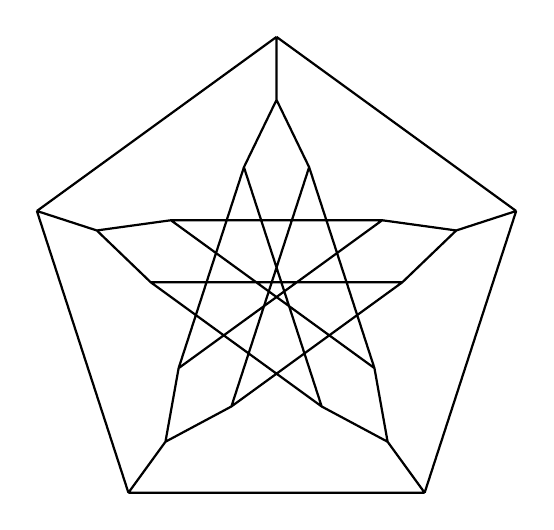
\begin{tikzpicture}[thick,scale=0.8]%
        \draw \foreach \x in {18,90,...,306} {
            (\x:4) node{} -- (\x+72:4)
            (\x:4) -- (\x:3) node{}
            (\x:3) -- (\x+15:2) node{}
            (\x:3) -- (\x-15:2) node{}
            (\x+15:2) -- (\x+144-15:2)
            (\x-15:2) -- (\x+144+15:2)
        };
    \end{tikzpicture}
\end{figure}

\end{document}
